\section{not sure yet}

\begin{definition}{CRC-32 nach IEEE 802.3}\\
    Wie können die Standards erreicht werden?\\
    Sicherung der Frames durch den CRC mit Polynom $x^0 + x^1 + ... + x^{32}$
    \begin{itemize}
        \item Minimale Hamming Distanz in Abhängigkeit der Frame-Länge:
        \begin{itemize}
            \item Bei der maximalen Distanz von 12000 Bit ist die minimale Hammingdistanz 4
            \item 3 Fehler können sicher erkannt werden
        \end{itemize}
    \end{itemize}
        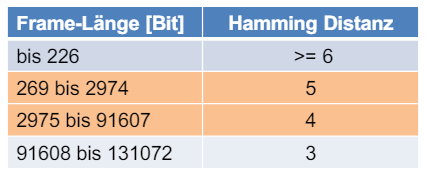
\includegraphics[width=0.5\linewidth]{images/CRC23_bsp.png}
\end{definition}

\begin{formula}{Berechnung der Restfehlerwahrscheinlichkeit}\\
    maximal F=3 Fehler bei einer Übertragung von N=12000 Bits
    $$P_{\leq F, N} = \sum_{t=0}^F \binom{N}{t} \cdot \epsilon^t \cdot (1 - \epsilon)^{N-t}$$
        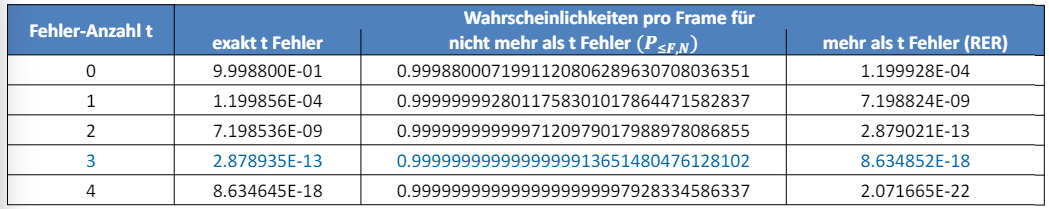
\includegraphics[width=1\linewidth]{images/fehlerwahrscheinlichkeit_berechnen.png}
\end{formula}

\begin{KR}{Worst Case Fehlererkennung für Ethernet}\\
    $5 \cdot 10^{-14}$ unentdeckte Fehler/Frame-Byte, max. BER = $10^{-8}$, max. $F_L$ = 1500 Bytes = 12000 Bit
    \begin{itemize}
        \item Wahrscheinlichkeit für fehlerhafte Frames:
    \end{itemize}
    $$P_{Fehler, Frame} \approx N \cdot p_e$$
    $12000 Bit \cdot 10^{-8} Fehler/Bit = 1.2 \cdot 10^{-4}$ : im Mittel ist jedes 8333. Frame fehlerhaft
    \begin{itemize}
        \item Wahrscheinlichkeit für unerkannte fehlerhafte Frames oberhalb Data Link Layer
    \end{itemize}
    $$RER \leq 1500 \frac{Bytes}{Frame} \cdot 5 \cdot 10^{-14} \frac{Fehler}{Byte} = 7.5 \cdot 10^{-11} \frac{Fehler}{Frame}$$
    ca. jedes 13'000'000'000 Frame ist unerkannt fehlerhaft
    \begin{itemize}
        \item Beispiel Backup 1.5 Tbyte:
    \end{itemize}
    $$1.5 \cdot 10^{12} Byte \cdot 5 \cdot 10^{-14} \frac{Fehler}{Byte} = 0.075 \frac{Fehler}{Backup}$$
    Jedes 13. Backup defekt!
    \begin{itemize}
        \item Beispiel Gigabit-Ethernet:
    \end{itemize}
    $$0.125 \cdot 10^9 \frac{Byte}{s} \cdot 5 \cdot 10^{-14} \frac{Fehler}{Byte} = 6.25 \cdot 10^{-6} \frac{Fehler}{s} = \frac{1 Fehler}{44h}$$
    Alle 44h ein unentdeckter Fehler!
\end{KR}